
\section{Building StanfordExtra: a new large-scale dog keypoint dataset}

\begin{figure*}[h]
    \centering
    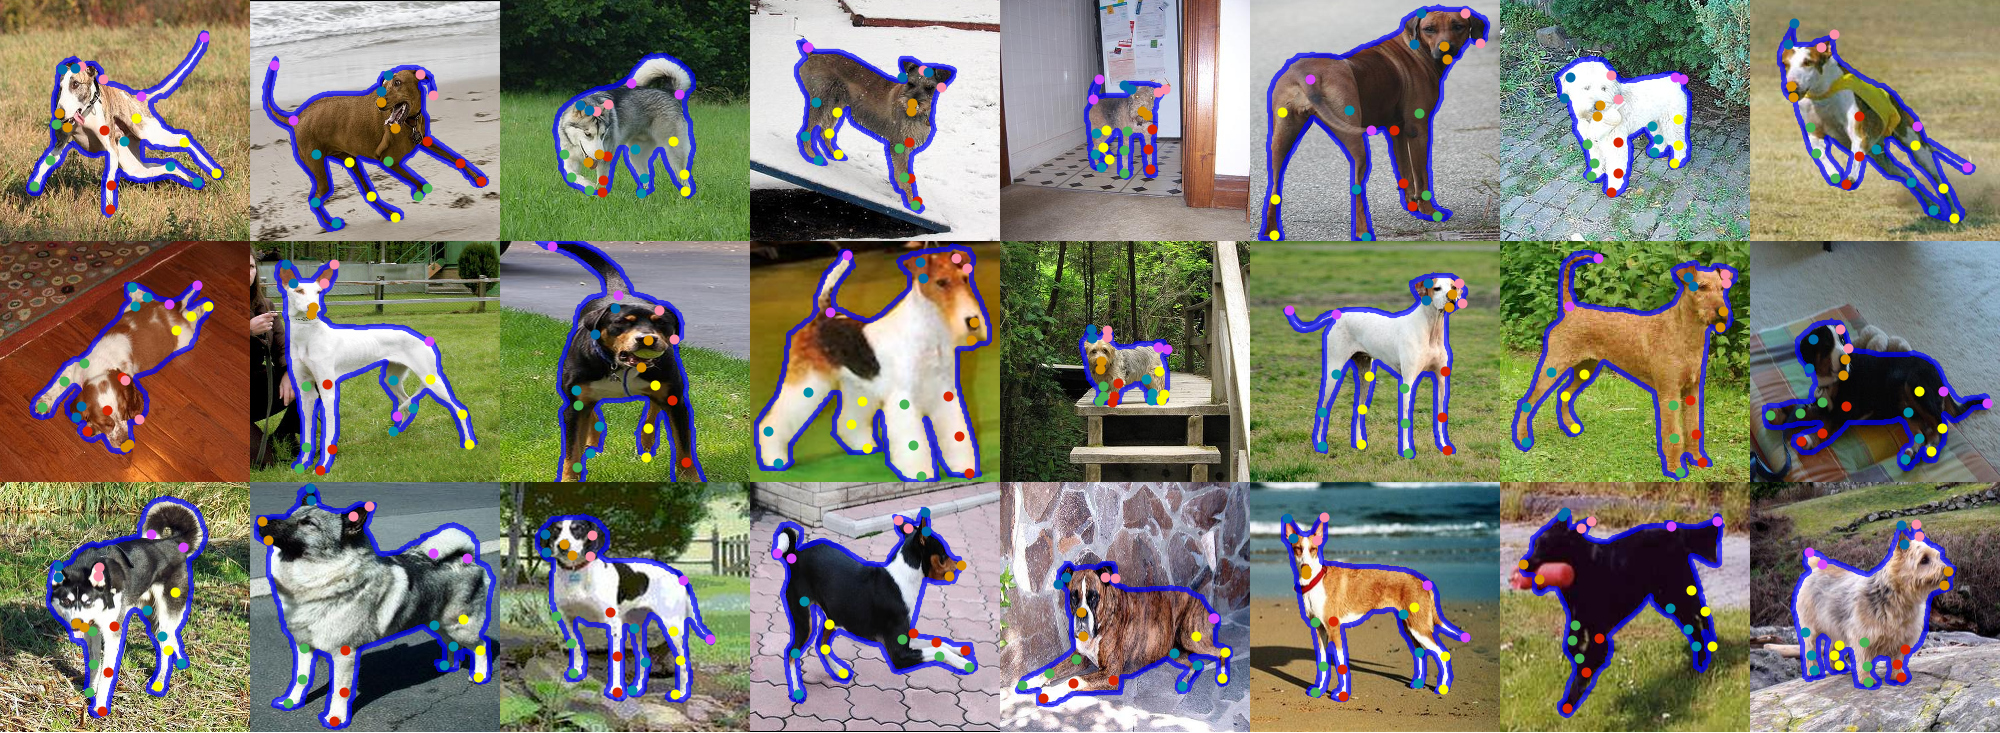
\includegraphics[height=0.1775\textheight]{OllieFigs/collage_wide.png}
    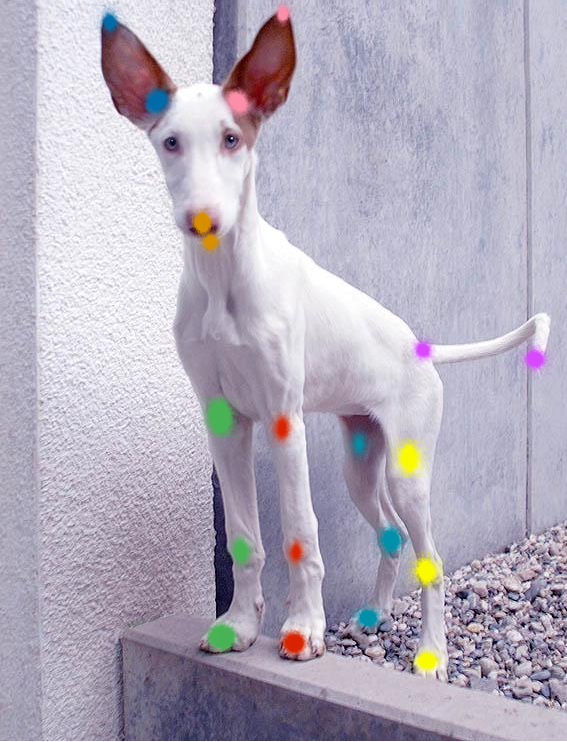
\includegraphics[height=0.1775\textheight]{OllieFigs/heatmap.png}
    \caption{\textbf{StanfordExtra example images}. \emph{Left}: outlined segmentations and labelled keypoints for 24 representative images. \emph{Right}: heatmap of deviation of worker submitted results from mean for each submission.}
    \label{fig:dataset}
\end{figure*}

In order to train and evaluate the method, it is neccessary to source a large-scale dataset of dog images with associated 2D annotations. This chapter therefore introduces \emph{StanfordExtra}: a new large-scale dataset with annotated 2D keypoints and binary segmentation masks for dogs. The source images were sourced from the existing Stanford Dog Dataset~\cite{StanfordDogs}, which consists of 20,580 dog images taken ``in the wild" and covers 120 dog breeds. The dataset contains vast shape and pose variation between dogs, as well as nuisance factors such as self/environmental occlusion, interaction with humans/other animals and partial views. Figure~\ref{fig:dataset} (left) shows samples from the new dataset.

Annotatations were collected using Amazon Mechanical Turk. The annotators (termed `turkers' on the platform) provided a binary silhouette mask and 20 keypoints per image. The remainder of this section describes the process for obtaining keypoint and segmentation annotations for the Stanford Dog Dataset~\cite{StanfordDogs}. 

The entire set of 20,580 dog images were first augmented with a single bounding box (provided with the original data) to indicate the largest dog in the image which the annotator should label. Each image was sent to 3 independent turkers with instructions explaining how to label the 20 keypoints and segmentation mask. 

\subsection{Keypoints.} 
Amazon turkers were given a list of 20 keypoints to click: 3 per leg (knee, ankle, toe), 2 per ear (base, tip), 2 per tail (base, tip), 2 per face (nose and jaw). They were additionally asked to provide a visibility flag per point. 

For each keypoint, we process the three clicks to yield a reliable coordinate. From the 3 clicks, we discard clicks that are further than a set tolerance from the mean. If at least 2 clicks remain, the mean coordinate is accepted as the keypoint position. Otherwise, the point has not been reliably identified so is set invisible. In line with other methods which tackle ``in-the-wild'' 3D reconstruction of articulated subjects~\cite{kolotouros19learning,kolotouros19convolutional}, images with fewer than a threshold number of visible keypoints (in this case 8 keypoints) are not included in StanfordExtra filtered from the dataset. This is since these images are unsuitable for the primary purpose of StanfordExtra, to train and evaluate full-body dog reconstruction task. 

% We rely on the following scheme to determine the optimal position of each keypoint, from the three annotations:

% \begin{enumerate}
%     \item 
% \end{enumerate}

% \begin{enumerate}
% \itemsep0em 
% \item{If If the keypoint was flagged highlighted by three different workers, and all three points are within a certain tolerance of the mean\footnote{Tolerance set at (Image width + Image height)/80, in pixels.}, then accept the mean as the keypoint position. If not, reject the furthest point from the mean, and go to step 2.}

% \item{If the keypoint was highlighted by two different workers, and both points are within a certain tolerance of the mean, accept the mean as the keypoint position. If not, reject the keypoint.}

% \item{If the keypoint was highlighted by only one worker, reject the keypoint.}

% \end{enumerate}


\subsection{Segmentation.}

\def\turker{t}
\def\turkertwo{t'}
\def\turkerboth{\bar{t}}

For each image, each worker $\turker \in \{\turker_{1}, \turker_{2}, \turker_{3}\}$ submits a binary segmentation mask $\mathbf{S}^{\turker}$. Submissions which fail simple criteria, such as if the segmentation area is below a threshold number of pixels, are sent for relabelling. 

% In order to sanitise the dataset and reduce erroneous entries, certain images were rejected or discarded. `Discarded' refers to a submission being discarded from the final dataset, whilst `rejected' means that the submission was deleted from the MTurk dataset, and a new entry requested from the website.\\

% As an initial pass, images were rejected (for which the bounding boxes were insufficiently large - to count null entries. For this, any entry was rejected if,

% \begin{equation}
% \sum\limits_{j=1}^H \sum\limits_{k=1}^W \mathbf{A}^{i,w}_{jk} < 0.01 WH 
% \end{equation}

For each image, the most likely segementation is generated by comparing submissions across workers. For any two turkers $\turker, \turkertwo$, a correlation coefficient is computed between submissions, summing over all pixels $i$. Note that $\bigotimes$ denotes the element-wise product of the matrices.

\begin{equation}
c(\turker, \turkertwo) = \frac{
    \sum_i \left[ \mathbf{S}^{\turker} \bigotimes \mathbf{S}^{\turkertwo} \right]_{i}}
    {\max\limits_{\turkerboth = \{\turker,\turkertwo\}} \sum_{i} \mathbf{S}^{\turkerboth}_{i}}
\end{equation}

% \begin{equation}
% c_{w,w'} = \frac{\mathbf{A}_{w} \odot \mathbf{A}_{w'}}{\max\limits_{p = \{w, w'\}}\mathbf{A}_{p}}
% \end{equation}

% We remove annotations for which all correlation coefficients are below 80\%. 
A worker's seggmentation $S^{\turker}$ is removed if all correlation coefficients $c(\turker,\turkertwo)$ are below a set threshold. The final binary mask is computed from the remaining submissions:

\begin{equation}
S^{*}_{i} = \begin{cases}
    1 & \text{if } \sum_{\turker} S^{\turker}_{i} > 1 \\
    0 & \text{otherwise}
\end{cases}
\end{equation}

\begin{figure}
\centering
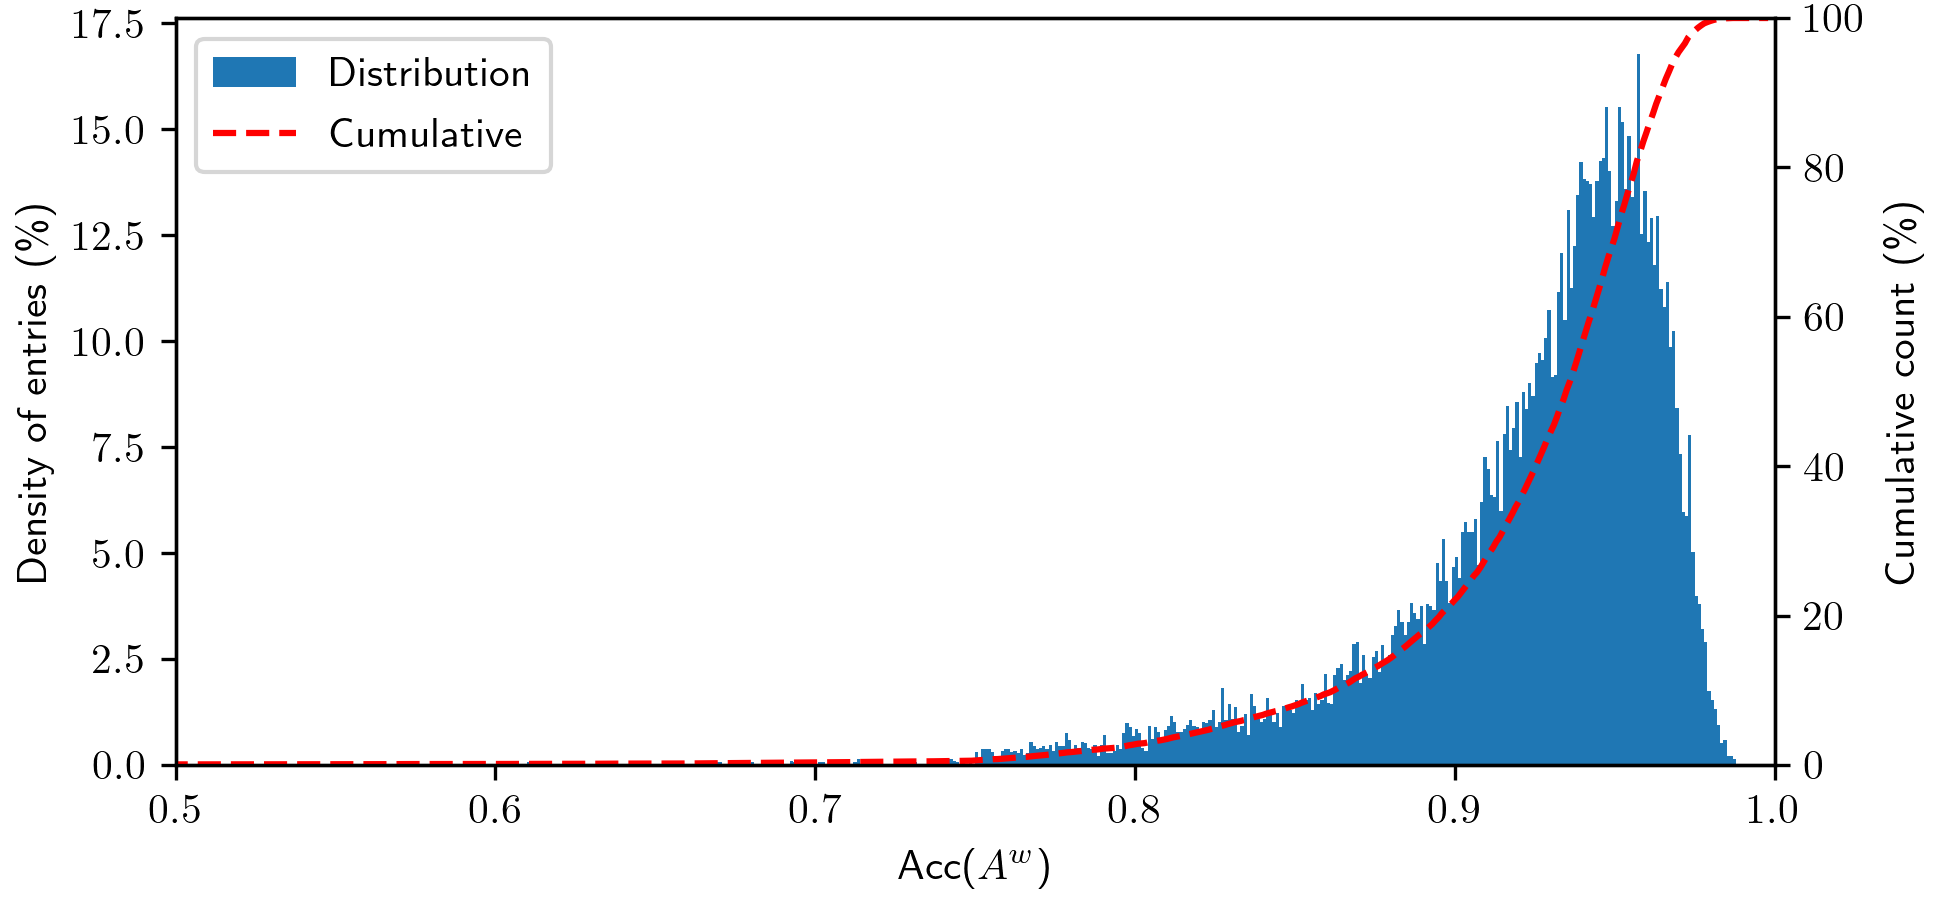
\includegraphics[width=0.95\textwidth]{OllieFigs/correlations.PNG}
\caption{Accuracy distribution of all submitted dog segmentations across the entire StanfordExtra dataset.}
\label{fig:accuracy distribution}
\end{figure}

With this, the accuracy of a worker's segmentation can be estimated according to the largest of their correlation coefficients: 

\begin{equation}
    \textrm{Acc}(S^{\turker})=\max_{\turkerboth \neq \turker} \{c(\turker, \turkerboth)\}
\end{equation}

\subsection{Approximating the dataset complexity.}

Figure~\ref{fig:dataset} gives an indication of the complexity of the dataset by analysing the distribution of worker accuracies across the entire StanfordExtra dataset.


% \subsubsection{Filtering the dataset.}

% As described in the paper, we reject images from our train/evaluation splits which based on reliability we deem unsuitable for our task of complete 3D reconstruction. have fewer than 8 identified keypoints find it necessary to reject The Stanford dog dataset contains 20,580 images. Not all of these images are constructive to this dataset - many do not have a lot of the dog in frame, etc. Several stages of refinement of the dataset were made, detailed in Table \ref{tab:filtering}.

% \begin{table}[]
%     \centering
%     \begin{tabular}{c|c}
%          \toprule
%          20,580 &  Stanford dataset\\
%          - (5,...) & Initial filtering based on bbox \\
%          - (5,...) & Images with fewer than 8 identified keypoints \\
%          - (60) & Images with insufficient segmentation accuracy \\
%          - (76) & Images for which more than one keypoint is outside of the segmentation\footnote{(with padding of 5 pixels)}\\
%          \midrule
%          9,647 & Final dataset\\
%          \bottomrule
%     \end{tabular}
%     \caption{Filtering process for final produced dataset}
%     \label{tab:filtering}
% \end{table}
